\documentclass[11pt,a4paper]{article}
\usepackage[utf8]{inputenc}
\usepackage[T1]{fontenc}
\usepackage{amsmath,amssymb,amsthm,mathrsfs}
\usepackage[margin=2.3cm]{geometry}
\usepackage{tikz}
\usetikzlibrary{arrows.meta,calc,patterns,positioning}
\usepackage[most]{tcolorbox}
\usepackage{enumitem}
\usepackage{xcolor}
\usepackage{fancyhdr}
\usepackage[hidelinks]{hyperref}

\definecolor{bleu}{RGB}{31,56,100}
\definecolor{bleuclair}{RGB}{47,85,151}
\definecolor{ocre}{RGB}{150,100,0}

% --- Macros mathématiques
\newcommand{\R}{\mathbb{R}}
\newcommand{\N}{\mathbb{N}}
\newcommand{\Q}{\mathbb{Q}}
\newcommand{\Rb}{\overline{\mathbb{R}}}
\newcommand{\A}{\mathscr{A}}
\newcommand{\B}{\mathscr{B}}
\newcommand{\C}{\mathscr{C}}
\newcommand{\M}{\mathscr{M}}
\newcommand{\Pp}{\mathscr{P}}
\newcommand{\Ee}{\mathscr{E}}
\newcommand{\Qq}{\mathscr{Q}}
\newcommand{\Ss}{\mathscr{S}}
\newcommand{\Oo}{\mathscr{O}}
\newcommand{\Ff}{\mathscr{F}}
\newcommand{\Ii}{\mathscr{I}}

% --- Mise en forme
\setlength{\parindent}{0pt}
\setlength{\parskip}{6pt}
\pagestyle{fancy}
\fancyhf{}
\renewcommand{\headrulewidth}{0.4pt}
\fancyhead[L]{\small\color{bleu}MAT361}
\fancyhead[R]{\small\color{bleu}Statistiques mathématiques}
\fancyfoot[C]{\thepage}

\newtcolorbox{enonce}[2]{enhanced,breakable,colback=bleuclair!6,colframe=bleuclair,
  boxrule=0pt,leftrule=3pt,arc=0pt,fonttitle=\bfseries\color{bleu},
  coltitle=bleu,title={#1~#2},attach boxed title to top left={yshift=-2mm},
  boxed title style={colback=white,colframe=white,boxrule=0pt,left=0pt,top=0pt,bottom=0pt},
  top=4pt,bottom=4pt}

\newtcolorbox{note}{enhanced,breakable,colback=yellow!8,colframe=ocre!70,
  boxrule=0pt,leftrule=2pt,arc=0pt,left=6pt,top=2pt,bottom=2pt,
  fontupper=\small\itshape,before upper={\textbf{\upshape[Note de transcription]}\ }}

\newenvironment{preuve}{\par\textit{\textbf{Preuve :}}\par\nopagebreak[4]}{\par}
\DeclareMathOperator{\sgn}{sgn}
\newcommand{\sect}[1]{\section*{#1}\addcontentsline{toc}{section}{#1}}
\newcommand{\datepage}[1]{\begin{flushright}\small\bfseries\itshape\color{bleuclair}#1\end{flushright}\vspace{-8pt}}

\newcommand{\PP}{\mathbb{P}}
\newcommand{\EE}{\mathbb{E}}
\newcommand{\ind}{\mathbf{1}}
\DeclareMathOperator{\Var}{Var}
\DeclareMathOperator{\Cov}{Cov}
\DeclareMathOperator*{\argmin}{arg\,min}
\begin{document}

\begin{center}
  {\Huge\bfseries\color{bleu} MAT361}\\[4pt]
  {\LARGE\bfseries\color{bleuclair} Statistiques mathématiques}\\[4pt]
  {\large\itshape Notes de cours saisies à partir du manuscrit}\\[6pt]
  {\normalsize\bfseries Lundi 12 octobre 2026}
\end{center}
\vspace{-4pt}
\hrule
\vspace{6pt}

\begin{note}
Les encadrés jaunes signalent une précision ajoutée ou une partie absente du manuscrit. Les lectures douteuses ont été remplacées par la version la plus probable. Le manuscrit n'est pas numéroté : les titres sont ceux du cahier et l'ordre des pages a été reconstitué par la logique du cours.
\end{note}

%=====================================================================
\section*{Rappel (1)}

\[
  \overline{\lim}\,u_n=\inf_{n}\ \sup_{k\ge n}u_k ,\qquad\qquad
  \underline{\lim}\,u_n=\sup_{n}\ \inf_{k\ge n}u_k .
\]

\subsection*{Lien avec le cours de Mesure}

\begin{center}
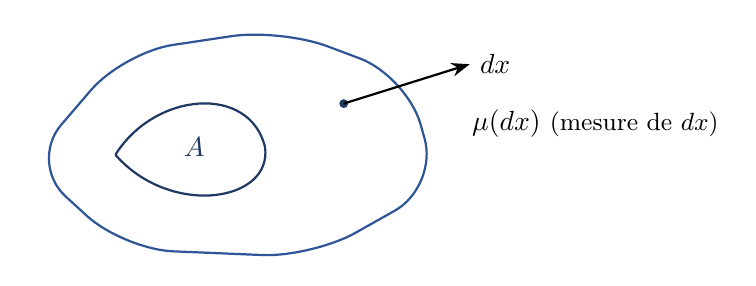
\begin{tikzpicture}[>=Stealth,thick]
  \draw[bleuclair,rounded corners=18pt] (0,0) -- (1.2,1.4) -- (3.2,1.7) -- (4.8,1.1) -- (5.2,-0.3) -- (3.6,-1.2) -- (1.2,-1.1) -- cycle;
  \draw[bleu] (1.1,0.1) .. controls (1.6,0.9) and (2.8,1.0) .. (3.0,0.2) .. controls (3.1,-0.5) and (1.8,-0.7) .. (1.1,0.1);
  \node[bleu] at (2.1,0.2) {$A$};
  \fill[bleu] (4.0,0.75) circle (1.6pt);
  \draw[->] (4.0,0.75) -- (5.6,1.25) node[right] {$dx$};
  \node[right] at (5.5,0.5) {$\mu(dx)$ \small(mesure de $dx$)};
\end{tikzpicture}
\end{center}

Pour $A\subset E$ :
\[
  \mu(A)=\int_A\mu(dx)=\int_A d\bigl(\mu(x)\bigr)=\int_E\ind_A\,d\mu(x)=\mu(A).
\]

\subsection*{Mesure de probabilité}

Soit $\mu:\Ff\to\Rb_+$ une mesure finie ($A\subset E$ ; $\mu(A)\le\mu(E)$, $\mu\ge0$). On définit
\[
  \PP:\ A\longmapsto\frac{\mu(A)}{\mu(E)} .
\]

%=====================================================================
\section*{Propriétés de continuité des probabilités}

Soit $(A_i)$ une suite d'événements et $B_i\subset A_i$ ; alors
\[
  \PP\Bigl(\bigcup A_i\Bigr)=\PP\Bigl(\bigcup B_i\Bigr)=\sum\PP(B_i)=\lim_{n\to+\infty}\sum_{i=1}^{n}\PP(B_i)\ \le\ \lim\sum_{i=1}^{n}\PP(A_i)=\sum\PP(A_i),
\]
puisque $\PP(B_i)\le\PP(A_i)$.

\textbf{\color{bleu}P6)} $(A_i)_{i\ge1}\nearrow$, c'est-à-dire $A_i\subset A_{i+1}$.
\[
  B_i=A_i\setminus\Bigl(\bigcup_{k<i}A_k\Bigr).
\]
$B_1=A_1$, $B_2=A_2\setminus A_1$, $B_1\cup B_2=A_1\cup(A_2\setminus A_1)=A_2$, \dots, $B_1\cup\dots\cup B_n=A_n$.
\[
  A_n=\bigcup_{i=1}^{n}B_i,\qquad \bigcup_{n\in\N}A_n=\bigcup_{n\in\N}\bigcup_{i=1}^{n}B_i=\bigcup_{i}B_i .
\]

Posons $B_1=A_1$, $B_i=A_i\cap\Bigl(\bigcup_{k\le i-1}A_k\Bigr)^c$.\\
$B_2=A_2\cap A_1^c$, \quad $B_3=A_3\cap(A_1\cup A_2)^c$.

\textbf{Montrons que les $B_i$ sont deux à deux disjoints.} Soit $i\neq j$ ; sans perte de généralité, $i<j$, c'est-à-dire $i\le j-1$.
\[
  B_j=A_j\cap\Bigl(\bigcup_{k=1}^{j-1}A_k\Bigr)^c,\qquad B_i=A_i\cap\Bigl(\bigcup_{l=1}^{i-1}A_l\Bigr)^c .
\]
Comme $i\le j-1$ : $A_i\subset A_{j-1}$, donc $A_i\cap A_{j-1}^c=\varnothing$. Alors
\[
  B_i\cap B_j=A_i\cap\Bigl(\bigcup_{k<i}A_k\Bigr)^c\cap A_j\cap\Bigl(\bigcap_{\substack{l<j\\ l\neq j-1}}A_l^c\Bigr)\cap A_{j-1}^c=\varnothing .
\]

\[
  B_1\cup B_2=A_1\cup[A_2\cap A_1^c]=(A_1\cup A_2)\cap\underbrace{(A_1\cup A_1^c)}_{=\Omega}=A_1\cup A_2 ,
\]
\[
  B_1\cup B_2\cup B_3=(A_1\cup A_2)\cup\bigl[A_3\cap(A_1\cup A_2)^c\bigr]
  =(A_1\cup A_2\cup A_3)\cap\bigl((A_1\cup A_2)\cup(A_1\cup A_2)^c\bigr)=A_1\cup A_2\cup A_3 .
\]

On a montré que $\displaystyle\bigcup A_i=\bigcup B_i$ avec $B_i\cap B_j=\varnothing$. Donc
\[
  \PP\Bigl(\bigcup A_i\Bigr)=\PP\Bigl(\bigcup B_i\Bigr)=\sum_{i=1}^{\infty}\PP(B_i)=\lim_{n\to+\infty}\sum_{i=1}^{n}\PP(B_i)
  =\lim_{n\to+\infty}\PP\Bigl(\bigcup_{i=1}^{n}B_i\Bigr)=\lim_{n\to+\infty}\PP(A_n).
\]

\textbf{\color{bleu}P7)} Soit $(A_i)\searrow$, c'est-à-dire $A_{i+1}\subset A_i\Rightarrow A_i^c\subset A_{i+1}^c\Rightarrow\{A_i^c\}\nearrow$, d'où
\[
  \PP\Bigl(\bigcup A_i^c\Bigr)=\lim_{n\to+\infty}\PP(A_n^c).
\]
Donc
\[
  \PP\Bigl[\Bigl(\bigcap A_i\Bigr)^c\Bigr]=1-\lim\PP(A_n),\qquad\text{et}\qquad 1-\PP\Bigl(\bigcap A_i\Bigr)=1-\lim\PP(A_i),
\]
soit $\PP\bigl(\bigcap A_i\bigr)=\lim\PP(A_i)$.

%=====================================================================
\section*{Mesure image}

Soit $T:(E,\Ff)\to(E',\Ff')$ mesurable et $\mu:\Ff\to\Rb_+$ une mesure.
\[
  \mu:\ \Ff\longrightarrow\Rb_+,\qquad A\longmapsto\mu(A),
\]
\[
  \mu_T:\ \Ff'\longrightarrow\Rb_+,\qquad A\longmapsto\mu_T(A)=\mu\bigl(T^{-1}(A)\bigr).
\]

\begin{note}
Le manuscrit s'arrête à « $\mu_T(A)=\mu($ » ; la définition est complétée par celle du cours de mesure.
\end{note}

%=====================================================================
\section*{Fonction de répartition}

\textbf{\color{bleu}$\ast$ Croissance.} Soit $x,y\in\R$ tels que $x\le y$. Montrons que $F_X(x)\le F_X(y)$.

On a : $F_X(x)=\PP(X\le x)$ et
\[
  (X\le x)=\{\omega\in\Omega\ /\ X(\omega)\le x\}\subset\{\omega\in\Omega\ /\ X(\omega)\le y\}\quad\text{car }x\le y .
\]
$\PP(X\le x)\le\PP(X\le y)$, donc $F_X(x)\le F_X(y)$.

\medskip
\textbf{\color{bleu}4)} \quad $\displaystyle\lim_{x\to-\infty}F_X(x)=\lim_{n\to+\infty}F_X(-n)$
\begin{align*}
  &=\lim_{n\to+\infty}\PP(X\le-n)=\lim_{n\to+\infty}\PP\bigl(X^{-1}(]-\infty;-n])\bigr)=\lim_{n\to+\infty}\PP_X\bigl(\underbrace{]-\infty;-n]}_{A_n}\bigr)\\
  &=\lim_{n\to+\infty}\PP(A_n)\ \text{ avec }(A_n)\searrow\\
  &=\PP_X\Bigl(\bigcap A_n\Bigr)=\PP_X(\varnothing)=\PP_X\bigl(X^{-1}(\varnothing)\bigr)=\PP(\varnothing)=0 .
\end{align*}

\begin{center}
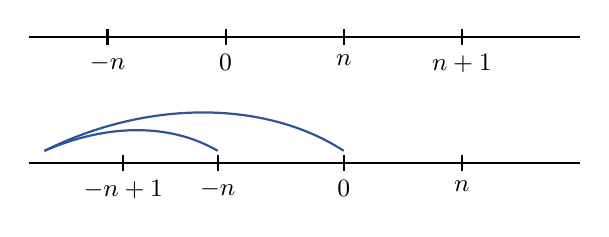
\begin{tikzpicture}[>=Stealth,thick,x=1cm,y=1cm]
  \draw (0,0) -- (7,0);
  \foreach \x/\l in {1/$-n$,2.5/$0$,4/$n$,5.5/$n+1$} {\draw (\x,0.1) -- (\x,-0.1) node[below,font=\small] {\l};}
  \begin{scope}[yshift=-1.6cm]
  \draw (0,0) -- (7,0);
  \foreach \x/\l in {1.2/$-n+1$,2.4/$-n$,4/$0$,5.5/$n$} {\draw (\x,0.1) -- (\x,-0.1) node[below,font=\small] {\l};}
  \draw[bleuclair] (0.2,0.15) .. controls (1.5,0.8) and (3,0.8) .. (4,0.15);
  \draw[bleuclair] (0.2,0.15) .. controls (1.0,0.5) and (1.8,0.5) .. (2.4,0.15);
  \end{scope}
\end{tikzpicture}
\end{center}

\textbf{\color{bleu}2) Continuité à droite.}
On veut montrer que $\displaystyle\lim_{x\to x_0^+}F_X(x)=F_X(x_0)$. On a :
\begin{align*}
  \lim_{x\to x_0^+}F_X(x)&=\lim_{n\to+\infty}F_X\Bigl(x_0+\frac1n\Bigr)\\
  &=\lim_{n\to+\infty}\PP\Bigl(X\le x_0+\frac1n\Bigr)=\lim_{n\to+\infty}\PP\Bigl(X^{-1}\bigl(]-\infty;x_0+\tfrac1n]\bigr)\Bigr)\\
  &=\lim_{n\to+\infty}\PP_X\Bigl(]-\infty;x_0+\tfrac1n]\Bigr).
\end{align*}
$n<n+1\Rightarrow\dfrac1{n+1}<\dfrac1n\Rightarrow A_{n+1}\subset A_n$ et $A_n\searrow$ :
\[
  =\PP_X\Bigl(\bigcap_{n}\,]-\infty;x_0+\tfrac1n]\Bigr).
\]
Soit $x\in\bigcap_n\,]-\infty;x_0+\frac1n]\Rightarrow\forall n$, $x\le x_0+\frac1n$. En passant à la limite, on a : $x\le x_0\Rightarrow x\in\,]-\infty;x_0]$.
Si $x\in\,]-\infty;x_0]$, $x\le x_0$ or $x_0\le x_0+\frac1n$ $\forall n$.

Donc $\displaystyle\bigcap_{n}\,]-\infty;x_0+\tfrac1n]=\,]-\infty;x_0]$.
\[
  \lim_{x\to x_0^+}F_X(x)=\PP_X\Bigl(\bigcap_n\,]-\infty;x_0+\tfrac1n]\Bigr)=\PP_X\bigl(]-\infty;x_0]\bigr)=\PP(X\le x_0)=F_X(x_0).
\]

\subsection*{Probabilité d'un intervalle}

$\blacksquare$\quad $\PP(a\le X<b)\neq\PP(a<X\le b)\neq\PP(a\le X\le b)$

\textit{Preuve.}

\underline{Cas 1 :} $\PP(a<X\le b)=F_X(b)-F_X(a)$.

\begin{center}
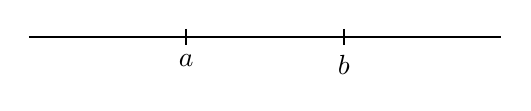
\begin{tikzpicture}[thick]
  \draw (0,0) -- (6,0);
  \draw (2,0.1) -- (2,-0.1) node[below] {$a$};
  \draw (4,0.1) -- (4,-0.1) node[below] {$b$};
\end{tikzpicture}
\end{center}

$]a,b]=\,]-\infty;b]\setminus\,]-\infty;a]$.
\begin{align*}
  \PP(a<X\le b)&=\PP_X\bigl(X^{-1}(]a,b])\bigr)=\PP_X(]a,b])\\
  &=\PP_X\bigl(]-\infty;b]\setminus\,]-\infty;a]\bigr)\\
  &=\PP_X(]-\infty;b])-\PP_X(]-\infty;a])\\
  &=\PP(X\le b)-\PP(X\le a)=F_X(b)-F_X(a).
\end{align*}

\underline{Cas 2 :} $\PP(a\le X<b)$. $\ [a,b[\,=\,]-\infty;b[\setminus\,]-\infty;a[$.
\begin{align*}
  \PP(a\le X<b)&=\PP_X([a,b[)\\
  &=\PP_X\bigl(]-\infty;b[\setminus\,]-\infty;a[\bigr)\\
  &=\PP_X(]-\infty;b[)-\PP_X(]-\infty;a[)\\
  &=\PP(X<b)-\PP(X<a)\\
  &=\lim_{x\to b^-}F_X(x)-\lim_{x\to a^-}F_X(x).
\end{align*}

%=====================================================================
\section*{Convergence d'une variable aléatoire}

\textbf{Pb :} On veut justifier le passage suivant
\[
  \lim_{n\to+\infty}\EE\bigl[f(X_n)\bigr]=\EE\Bigl(\lim_{n\to+\infty}f(X_n)\Bigr).
\]

\textbf{\color{bleu}Rappels :} notion de convergence de la V.A.

En $\R$ : $u_n\to u\iff\forall\varepsilon>0$, $\exists n_\varepsilon\in\N$, $n\ge N_\varepsilon\Rightarrow|u_n-u|<\varepsilon$.

Si $\{X_n\}$ est une suite de V.A, alors comment comprendre $X_n\to X$ ?

On pourrait penser à écrire
\[
  X_n\to X\ \text{ ssi }\ \forall\varepsilon>0,\ \exists n_\varepsilon\in\N\ /\ n\ge N_\varepsilon\Rightarrow|X_n-X|<\varepsilon .
\]
\textbf{Difficulté} (mode de convergence en probabilité) :
\begin{enumerate}[label=\textbf{\roman*)},leftmargin=1.2cm]
  \item $|X_n-X|$ est un évènement ;
  \item $|X_n-X|<\varepsilon\Rightarrow\{\omega\in\Omega\ /\ |X_n(\omega)-X(\omega)|<\varepsilon\}$ ;
  \item c'est un évènement et dire que $A_n$ se réalise avec une certaine probabilité.
\end{enumerate}

\subsection*{1\textsuperscript{er} mode de convergence}

\begin{enonce}{Convergence}{en probabilité}
\[
  X_n\xrightarrow{\ \PP\ }X\iff\forall\varepsilon>0,\ \exists n_\varepsilon\in\N,\quad n\ge N_\varepsilon\Rightarrow\PP(|X_n-X|<\varepsilon)\to1 .
\]
\end{enonce}

Comme $\PP(|X_n-X|<\varepsilon)=1-\PP(|X_n-X|\ge\varepsilon)$, on a de façon équivalente :
\[
  X_n\xrightarrow{\ \PP\ }X\iff\forall\varepsilon>0,\ \lim_{n\to+\infty}\PP(|X_n-X|>\varepsilon)=0 .
\]

\subsection*{2\textsuperscript{ème} mode (convergence presque sûre)}

\[
  X_n\xrightarrow{\ \text{p.s}\ }X\ \text{ ssi }\ \PP\bigl(\lim X_n=X\bigr)=1
\]
ssi $\exists\,\Omega_1\subset\Omega$ tel que $\PP(\Omega_1)=1$ et $\forall\omega_0\in\Omega_1$, $\displaystyle\lim_{n\to+\infty}X_n(\omega_0)=X(\omega_0)$.

Avec $\PP(\Omega\setminus\Omega_1)=0$ et $\forall\omega_0\in\Omega\setminus\Omega_1$, $\displaystyle\lim_{n\to+\infty}X_n(\omega_0)\neq X(\omega_0)$ (ou la limite n'existe pas).

\subsection*{3\textsuperscript{ème} mode (convergence en distribution)}

Soit $(X_n)$ une suite de V.A de fonction de répartition $F_{X_n}$.
\[
  X_n\xrightarrow{\ d\ }X\iff F_{X_n}(x)\longrightarrow F_X(x),\qquad\forall x\in F_X^{\,c}\ \ (\text{point de continuité de }F_X).
\]

%=====================================================================
\section*{Lois limites}

\textbf{\color{bleu}$\bullet$ LFGN} (loi faible des grands nombres). Si $(X_i)$ est une suite de V.A telle que $\EE(X_1)<+\infty$ et les $X_i$ sont iid, i.e.\ $\mu=\EE(X)$, $\sigma^2=\Var(X)$.
Alors
\[
  \frac1n\sum X_i\xrightarrow{\ \PP\ }\EE(X_1).
\]

\textbf{\color{bleu}$\bullet$ LPGN} (loi forte des grands nombres). $(X_i)$ iid telle que $\EE(X_i^{+})<+\infty$, $\mu=\EE(X_i)$, $\sigma^2=\Var(X_i)$ ; alors
\[
  \frac1n\sum X_i\xrightarrow{\ \text{p.s}\ }\EE(X_1).
\]

\textbf{\color{bleu}$\bullet$ TCL.} Si on a $(X_i)$ iid de moyenne $\mu=\EE(X_i)$, $\sigma^2=\Var(X_i)$ :
\[
  \sqrt n\,(\overline X_n-\mu)\xrightarrow{\ d\ }\mathcal N(0,\sigma^2).
\]
De même,
\[
  \frac{\sqrt n\,(\overline X_n-\mu)}{\sigma}\xrightarrow{\ d\ }\mathcal N(0,1),\qquad\text{où }\ \overline X_n=\frac1n\sum_{i=1}^{n}X_i .
\]

\begin{note}
La page « Lois limites » n'est reliée aux autres par aucune phrase ; elle est placée après les trois modes de convergence, dont elle utilise les notations.
\end{note}

%=====================================================================
\section*{Passage de la limite dans l'espérance}

On veut répondre à la question du passage de la limite dans l'espérance.

\textbf{3 résultats principaux :}
\begin{enumerate}[label=\textbf{(\roman*)},leftmargin=1.2cm]
  \item Beppo-Levi ;
  \item Convergence dominée ;
  \item Lemme de Fatou.
\end{enumerate}

\textbf{(i)} Si $X_n\nearrow$ ou $X_n\searrow$ tel que $X_n\to X$, on montre que (B.~Levi)
\[
  \lim_{n\to+\infty}\EE\bigl(f(X_n)\bigr)=\EE\bigl(\lim_n f(X_n)\bigr).
\]

\textbf{(ii) \underline{Convergence dominée.}} Soit $(X_n)_n$ une suite de V.A telle que $X_n\to X$ et il existe $Y$ tel que $|X_n|\le Y$ avec $Y\in L^1$
(espérance de valeur absolue est finie). Alors
\[
  \lim\EE\bigl(f(X_n)\bigr)=\EE\bigl(\lim f(X_n)\bigr).
\]

\begin{note}
Le lemme de Fatou (iii) est annoncé mais n'est pas développé dans le manuscrit.
\end{note}

%=====================================================================
\section*{Inégalité de Markov}

Soit $A\subset\Omega$ ; $\ind_A=\begin{cases}1&\text{si }x\in A\\0&\text{sinon}\end{cases}$, $\ \ind_\Omega=1$ \qquad(l'indicatrice est positive).

Soit $X$ une V.A positive et $a>0$.
\[
  X=X\times1=X\ind_\Omega .
\]
$\Omega=\{X<a\}\cup\{X\ge a\}$, donc
\[
  \ind_\Omega=\ind_{\{X<a\}}+\ind_{\{X\ge a\}},
\]
\[
  X\ind_\Omega=\underbrace{X\ind_{\{X<a\}}}_{\ge0}+X\ind_{\{X\ge a\}} .
\]
$X\ind_\Omega\ge X\ind_{\{X\ge a\}}$.
\[
  X\ge X\ind_{\{X\ge a\}}\ge a\ind_{\{X\ge a\}}\ \Longrightarrow\ X\ge a\ind_{\{X\ge a\}} .
\]

\textbf{Rappel :} (lien entre $\EE$ et $\PP$)
\[
  \PP(A)=\int_A d\PP=\int_\Omega\ind_A\,d\PP=\EE[\ind_A].
\]

D'où
\[
  X\ge a\ind_{\{X\ge a\}}\Rightarrow\EE(X)\ge a\,\EE\bigl(\ind_{\{X\ge a\}}\bigr)\Rightarrow\EE(X)\ge a\,\PP(X\ge a).
\]

\begin{enonce}{Inégalité}{de Markov}
\[
  \PP(X\ge a)\le\frac{\EE(X)}{a}.
\]
\end{enonce}

Si $X$ est une V.A quelconque, on pose $Y=|X|\ge0$, $a>0$ :
\[
  \PP(|X|\ge a)\le\frac{\EE|X|}{a},\qquad\PP(X^2\ge a^2)\le\frac{\EE(X^2)}{a^2}.
\]

Soit $X$ une V.A telle que $\EE(X)=\mu$ et $\Var(X)=\sigma^2$.
$Y=|X-\EE(X)|$.
\[
  \PP\bigl(|X-\EE(X)|\ge a\bigr),\ a>0\ =\ \PP\bigl(|X-\EE(X)|^2\ge a^2\bigr)\ \le\ \frac{\EE\bigl(|X-\EE(X)|^2\bigr)}{a^2}=\frac{\Var(X)}{a^2}=\frac{\sigma^2}{a^2}.
\]

\begin{note}
Le manuscrit alterne les écritures $\{X>a\}$ et $\{X\ge a\}$ ; j'ai uniformisé avec $\{X\ge a\}$, forme usuelle de l'inégalité de Markov. La mention « $\mu=\PP$ » écrite dans l'en-tête de la feuille n'est pas transcrite.
\end{note}

%=====================================================================
\section*{Inégalité de Cauchy-Schwarz}

\[
  \Bigl|\sum u_iv_i\Bigr|\le\sqrt{\Bigl(\sum u_i^2\Bigr)\Bigl(\sum v_i^2\Bigr)}.
\]
Soit $X,Y$ deux variables aléatoires.
\[
  \int|X|\cdot|Y|\,d\PP\le\sqrt{\int X^2\,d\PP\cdot\int Y^2\,d\PP}.
\]
Mieux encore,
\[
  \int|X-\EE(X)|\,|Y-\EE(Y)|\,d\PP\le\sqrt{\int\bigl(X-\EE(X)\bigr)^2d\PP}\times\sqrt{\int\bigl(Y-\EE(Y)\bigr)^2d\PP}
\]
\[
  \EE\bigl[|X-\EE(X)|\,|Y-\EE(Y)|\bigr]\le\sqrt{\Var(X)\Var(Y)}
\]
\[
  |\Cov(X,Y)|\le\sqrt{\Var(X)\Var(Y)},\qquad\Biggl|\frac{\Cov(X,Y)}{\sqrt{\Var(X)\Var(Y)}}\Biggr|\le1 .
\]

%=====================================================================
\section*{Paramètre de position}

On se place sur $(\Omega,\A,\PP)$. $X:\Omega\to\R$,
\[
  \EE(X)=\EE_{\PP}(X)=\int_\Omega X\,d\PP .
\]
Théorème de transfert : $\displaystyle\EE(X)=\int_\Omega X\,d\PP=\int_\R x\,d\PP_X(x)$.

On montre que
\[
  \mu_X=\argmin_{c\in\R}\ \EE\bigl[(X-c)^2\bigr].
\]
On pose $\varphi(c)=\EE\bigl[(X-c)^2\bigr]$
\begin{align*}
  &=\EE\bigl(X^2-2cX+c^2\bigr)\\
  &=\EE(X^2)-2c\,\EE(X)+c^2 ,
\end{align*}
$\varphi'(c)=-2\,\EE(X)+2c$, $\ \varphi''(c)=2>0$,\\
$\varphi'(c)=0\iff c=\EE(X)$.

\begin{note}
La page est photographiée en travers dans l'original ; elle a été redressée dans le PDF réorganisé.
\end{note}

\end{document}
